\subsection{Product perspective} 
The product we will develope is a software application  for smartphone implementing Android as operative system. The app will require the user to be registered in order to access to all the funtionalities. It will also need a stable internet connection in order to connect to different external system providing information about weather and transport means. The application runs locally on the smartphone but users data are also stored in the the system database.

\begin{figure}[!h]
	\centering
	\makebox[\textwidth][c]{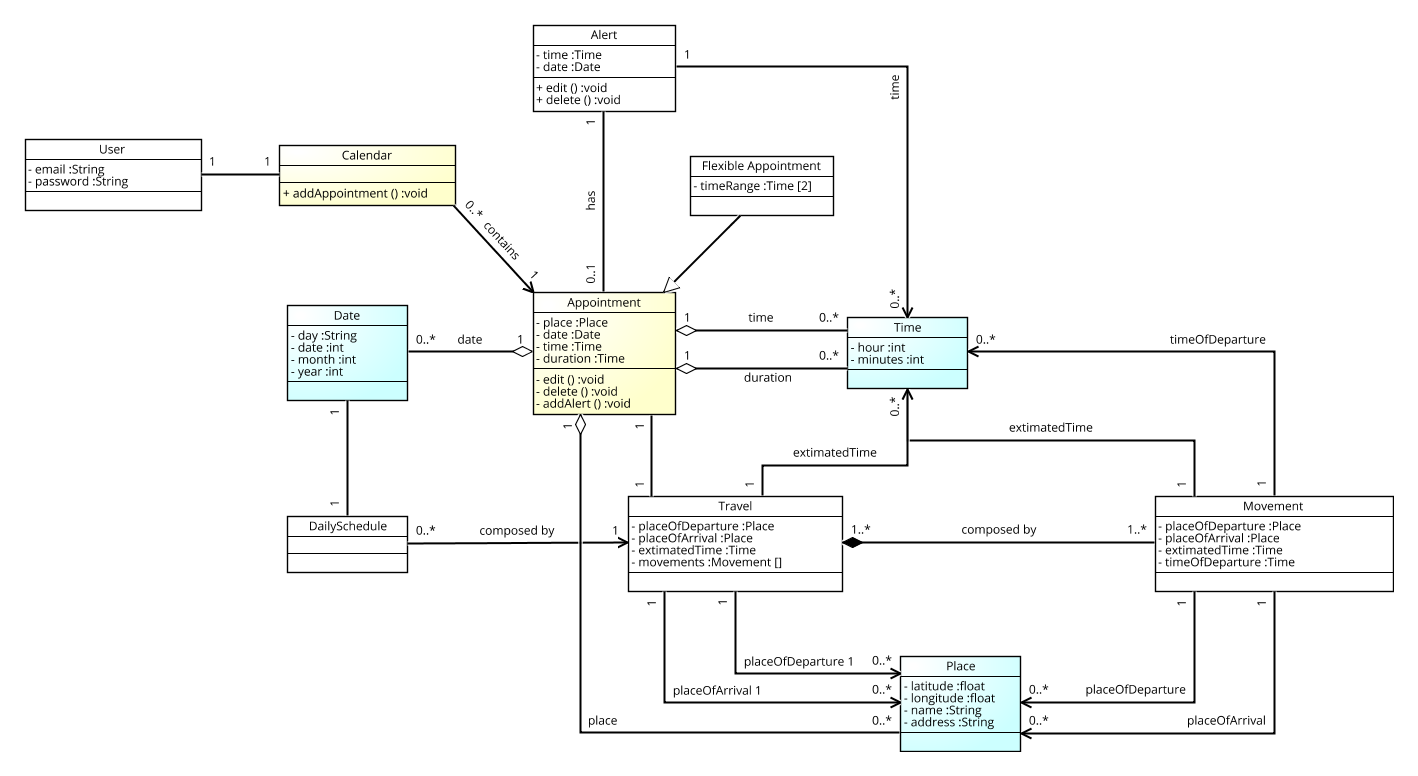
\includegraphics[width=1.2\textwidth]{Images/ClassDiagram.png}}%
\end{figure}

\subsection{Product functions}
This application aims to provide a smart and user-friendly appointment-manager system, which allows the user to create and keep track of several appointment on a personal virtual calendar. Plus, the app is able to schedule the travels to reach the different appointment destinations on time in the fastest and most confortable way, according to the preferences expressed by the user and the different weather and public transport condition. Finally, the application offers the possibility of easily buy tickets for the different trips, and to view them when needed.
\subsection{User characteristics}
We recommend this application to a everyone who wants to easily manage his appointments without any loss of time. The app is designed to be as user friendly as possible, so the user is not forced to have a specific knowledge of the system to be able to benefit of the service. It can be used by a business man with a calendar full of work meetings or just by an ordinary student to schedule his study breaks. Furthermore, the possibility of buying tickets suits even simple travelers who need to manage their trips.
\subsection{Dependencies}
\begin{itemize}
	\item The application requires a stable internet connection, by Wi-Fi or mobile network.
	\item The application makes use of GPS localization to access to the user position.
	\item Based on the user choice, the application may require a connection to an existing Facebook or Google account.
	\item The application makes use of external APIs to achieve information about maps, public transport and weather condition.
	\item The application depends entirely on the ATM and Trenord public transport Payment Service for everything concerning the tickets purchase.
\end{itemize}
\subsection{Constrains}
\begin{itemize}
	\item The application requires the user to be registred and logged into the system to work properly.
	\item The application works only on smartphones that implement Android version 4.0.3 or later.
	\item The application is in beta version and works only inside the urban area of Milan.
	\item 30 Mb(?) of storage memory must be available on the device in order to correctly install the application.
\end{itemize}


